    \begin{wrapfigure}{R}{0.5\textwidth}
   \begin{center}
    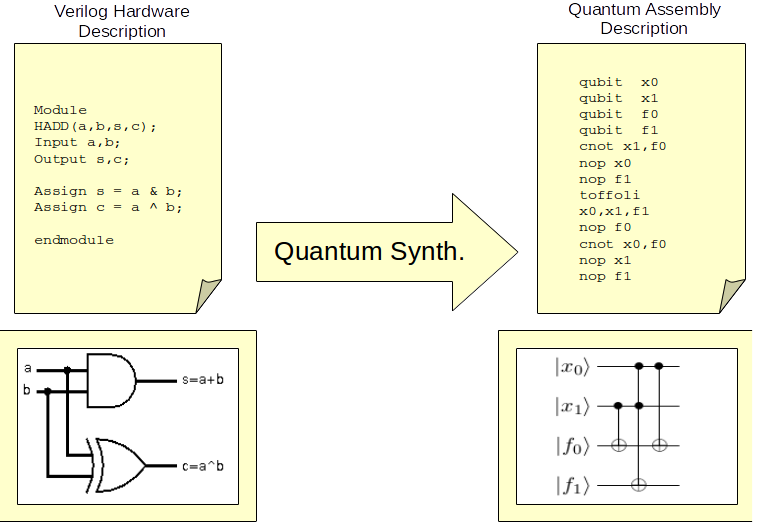
\includegraphics[width=0.48\textwidth]{QuantumSynthesis.png}
  \end{center}
\end{wrapfigure}
One advantage to this project is that a tool which can handle the synthesis of quantum designs given a verilog specification has already been developed. 
As part of the project, this tool will be refined, and utilized to synthesize verilog descriptions of numerical methods into their equivalent quantum forms. 
We will then use an existing quantum simulator to evaluate the speedups that are experienced when using a quantum method for the solution. 
The tool was developed by Micah Thornton, and relies on some previous packages that were developed at other universities such as Berkeley and MIT. 
A pictoral representation of the tool is here: 

    %\begin{figure} [h!]
      %  \centering
     %   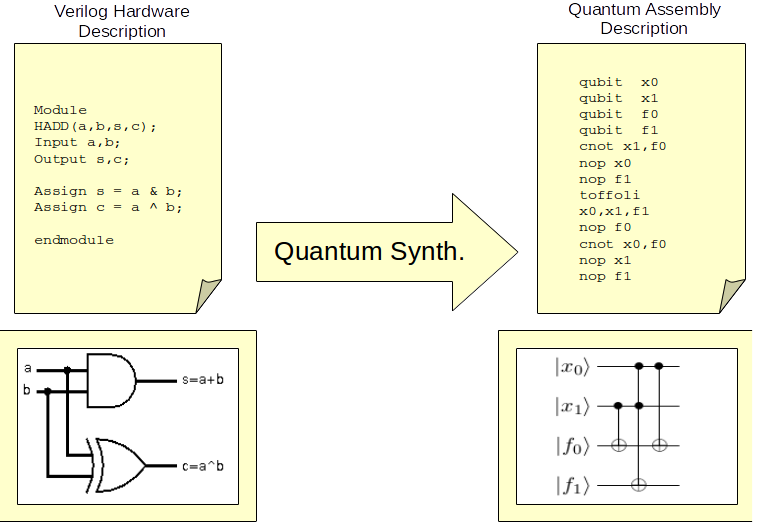
\includegraphics[scale = 0.35]{QuantumSynthesis.png}
    %\end{figure}

